% V-model
\subsection{Approach}
This work has been implemented with an adaptation of V-model development process
\footnote{Described in detail here: \cite{mathur2010advancements}}.
The original version of this process is known as a variation of the waterfall process,
with several phases that resembles the latter,
but the their displacement is slightly modified,
emphasising on the coding phase.

An appealing feature of the V-model is that every phase,
before the coding one,
has a 1:1 strong relationship with the phases that occurs after the coding,
reinforcing the mapping of the theoretical part of the project with the practical one.
Moreover,
in comparison with Agile models,
there is much more documentation in a project using V-model,
and this feature is crucial for this work.

The adaptation made in this project was to divide the V-model into iterations separated by the use cases.
That is,
for every use case,
there are the execution of every phase of V-model,
as if the product would have only one use case.

Curiously,
after some research about the flaws of V-model,
a variation of the V-model has been found and it shares the fundamental difference between this work's approach and V-model:
the Dual V-model \cite{clark2009system}.
The shared idea is: divide and conquer V-model, 
by making subsystems that follows V-model,
so,
when these subsystems are finished,
they can be integrated to create the final product.

% \subsubsection{How it works}

FIGURE V-MODEL

% \subsubsection{Mapping V-model to this work}
\begin{description}
    \item[Requirements Analysis] Sections \ref{sec:useCases} and \ref{sec:requirements}
    \item[Specification / System Design] Section \ref{sec:design}
    \item[Architectural Design / System Architecture] Section  \ref{sec:architecture}
    \item[Detail Design / Module Design] Section \ref{implementation}
    \item[Unit Testing] 
    \item[Integration Testing] 
    \item[System Testing] 
    \item[User Acceptance Testing] Not used, because we are building a proof of concept.
\end{description}


\subsection{Use Cases}
\label{sec:useCases}
%Sometimes it is a good idea to put domain objects in \texttt{}
%The template and the descriptions are based on the book Applying UML and Patterns: 
%An Introduction to Object-Oriented Analysis and Design and Iterative Development
%(3rd Edition) by Craig Larman.
\begin{usecase}

\addtitle{Water cycle control}{Template test} 

%Scope: the system under design
%\addfield{Scope:}{System-wide}

%Level: "user-goal" or "subfunction"
%\addfield{Level:}{User-goal}

%Primary Actor: Calls on the system to deliver its services.
\addfield{Actors:}{Microcontroller}

%Stakeholders and Interests: Who cares about this use case and what do they want?
%\additemizedfield{Stakeholders and Interests:}{
	%\item Stakeholder 1 name: his interests
	%\item Stakeholder 2 name: his interests
%}

%Preconditions: What must be true on start and worth telling the reader?
%\addfield{Preconditions:}{}
%when multiple
\additemizedfield{Preconditions:}{
    \item The Microcontroller must be installed in the system
    \item A proper relay must be installed in the system
    \item The external power supply and the water pump must be compatible
    %\item Water pump and the PWM module are working normally
} 

%Postconditions: What must be true on successful completion and worth telling the reader
\addfield{Postconditions:}
{
    The fish tank's water should be pumped to the vegetable media each quarter of an hour.
}
%when multiple
%\additemizedfield{Preconditions:}{}

%Main Success Scenario: A typical, unconditional happy path scenario of success.
\addscenario{Main Success Scenario:}{
	\item The Microcontroller executes a run cycle of 25\% in a 1 hour period.
	%\item The Microcontroller executes a run cycle of 25\% in the PWM in a 1 hour period.
	\item The circuit sends this signal to a relay.
    \item The relay activates the water pump at a 15 minutes per hour rate with the adequate voltage.
}

%Extensions: Alternate scenarios of success or failure.
%\addscenario{Extensions:}{
	%\item[2.a] Invalid login data:
		%\begin{enumerate}
		%\item[1.] System shows failure message
		%\item[2.] User returns to step 1
		%\end{enumerate}
	%\item[5.a] Invalid subsriber data:
		%\begin{enumerate}
		%\item[1.] System shows failure message
		%\item[2.] User returns to step 2 and corrects the errors
		%\end{enumerate}
%}

%Special Requirements: Related non-functional requirements.
\additemizedfield{Special Requirements:}{
	%\item R1: Operation Time Limit requirement
	\item \ref{req1}
}

% TODO: COOL Technology and Data Variations List: Varying I/O methods and data formats.
%\addscenario{Technology and Data Variations List:}{
	%\item[1a.] Alternative first action with other technology
%}

%Frequency of Occurrence: Influences investigation, testing and timing of implementation.
%\addfield{Frequency of Occurrence:}{}

%Miscellaneous: Such as open issues/questions
%\addfield{Open Issues:}{}

\end{usecase}

%Sometimes it is a good idea to put domain objects in \texttt{}
%The template and the descriptions are based on the book Applying UML and Patterns: 
%An Introduction to Object-Oriented Analysis and Design and Iterative Development
%(3rd Edition) by Craig Larman.
\begin{usecase}

\addtitle{Keep water tank's pH level in 6-7 range}{Details} 

%Scope: the system under design
%\addfield{Scope:}{System-wide}

%Level: "user-goal" or "subfunction"
%\addfield{Level:}{User-goal}

%Primary Actor: Calls on the system to deliver its services.
\additemizedfield{Actors:}
{
\item Microcontroller
\item Peristaltic Water Pumps 
\item pH Sensors
}

%Stakeholders and Interests: Who cares about this use case and what do they want?
%\additemizedfield{Stakeholders and Interests:}{
	%\item Stakeholder 1 name: his interests
	%\item Stakeholder 2 name: his interests
%}

%Preconditions: What must be true on start and worth telling the reader?
%\addfield{Preconditions:}{}
%when multiple
\additemizedfield{Preconditions:}{
    \item The Microcontroller, pH sensors and the peristaltic pumps must be installed in the system
    \item A proper relay must be installed in the system
         OR a power transistor to supply 12V DC
    \item The external power supply and the water pump must be compatible
} 

%Postconditions: What must be true on successful completion and worth telling the reader
\addfield{Postconditions:}
{
    The water tank's pH level is between 6 and 7.
}
%when multiple
%\additemizedfield{Preconditions:}{}

%Main Success Scenario: A typical, unconditional happy path scenario of success.
\addscenario{Main Success Scenario:}{
	\item The Microcontroller checks the pH sensor.
    \item The pH output is between 6 and 7.
	%\item The Microcontroller executes a run cycle of 25\% in the PWM in a 1 hour period.
}

%Extensions: Alternate scenarios of success or failure.
\addscenario{Extensions:}{
	\item[2.a] Lower pH values in output:
		\begin{enumerate}
            \item[1.] The circuit sends this signal to start the high pH relay.
            \item[2.] The relay distributes the needed current to the high pH's peristaltic pump.
            \item[3.] High pH water is blended with the water tank's, until the latter gets into the normal pH range.
            \item[1.] The circuit sends this signal to stop the high pH relay.
		%\item[2.] User returns to step 1
		\end{enumerate}
	\item[2.a] Higher pH values in output:
		\begin{enumerate}
            \item[1.] The circuit sends this signal to start the low pH relay.
            \item[2.] The relay distributes the needed current to the low pH's peristaltic pump.
            \item[3.] High pH water is blended with the water tank's, until the latter gets into the normal pH range.
            \item[1.] The circuit sends this signal to stop the low pH relay.
		%\item[2.] User returns to step 1
		\end{enumerate}
	%\item[5.a] Invalid subsriber data:
		%\begin{enumerate}
		%\item[1.] System shows failure message
		%\item[2.] User returns to step 2 and corrects the errors
		%\end{enumerate}
}

%Special Requirements: Related non-functional requirements.
\additemizedfield{Special Requirements:}{
	%\item R1: Operation Time Limit requirement
	\item \ref{req2}
}

% TODO: COOL Technology and Data Variations List: Varying I/O methods and data formats.
%\addscenario{Technology and Data Variations List:}{
	%\item[1a.] Alternative first action with other technology
%}

%Frequency of Occurrence: Influences investigation, testing and timing of implementation.
%\addfield{Frequency of Occurrence:}{}

%Miscellaneous: Such as open issues/questions
%\addfield{Open Issues:}{}

\end{usecase}


\subsubsection{Summary table}

\begin{table}[h]
\centering
\caption{Requirements table}
\label{tab:requirementsTable}
\begin{tabular}{|c|c|c|}
\hline
\textbf{Use Case}    & \textbf{Requirement} & \textbf{References} \\ \hline
Optimize Water Cycle & \ref{req1}           &                 \\ \hline
Keep pH Level optimum & \ref{req2}           &  \cite{tables} \\ \hline
\end{tabular}
\end{table}

\subsection{Requirements}
\label{sec:requirements}

\begin{description}

\item [\req{1}]
Optimize the water cycle period between fish tank and plants medium.

\item [\req{2}]
Keep the pH Level around the 6-7 range.

\end{description}

\subsection{System Design}
\label{sec:design}

The figure \ref{fig:highLevelSystemDesign} shows a high level diagram to demonstrate how the automation can be implemented in the Aquaponics.
Each node has an input and output,
indicated by an incoming and outgoing arrows, respectfully.

The components are from the original Aquaponics system,
which are surveyed by the sensors.
The latter captures dedicated data from the medium,
like temperature or water level and emits an electronic signal to the microcontroller.

The latter is the main responsible for the automation,
it is where the logic is stored,
so the input signal are interpreted by the installed program and another electronic signal is sent to the components,
this signal could be directed or indirect,
the former is when the output current is enough to the target component to work,
otherwise the latter is used via a relay,
that is connected with an external power supply,
and behaves as an signal amplifier.

\begin{figure}[h]
    \centering
    \includegraphics[width=.7\linewidth]{diagrams/systemDesign}
    \caption{A simple diagram to represent a high level design of this project}
    \label{fig:highLevelSystemDesign}
\end{figure}

\subsection{System Architecture}
\label{sec:architecture}

At the figure \ref{sec:architecture} the low-level design is illustrated.
Based on the figure \ref{fig:highLevelSystemDesign},
the figure \ref{fig:waterCycleDiagram} depicts a model to automatize the water cycle control from the requirement \ref{req1}.
Now one can see where to connect each terminal and every important component is presented.

\begin{figure}[h]
    \centering
    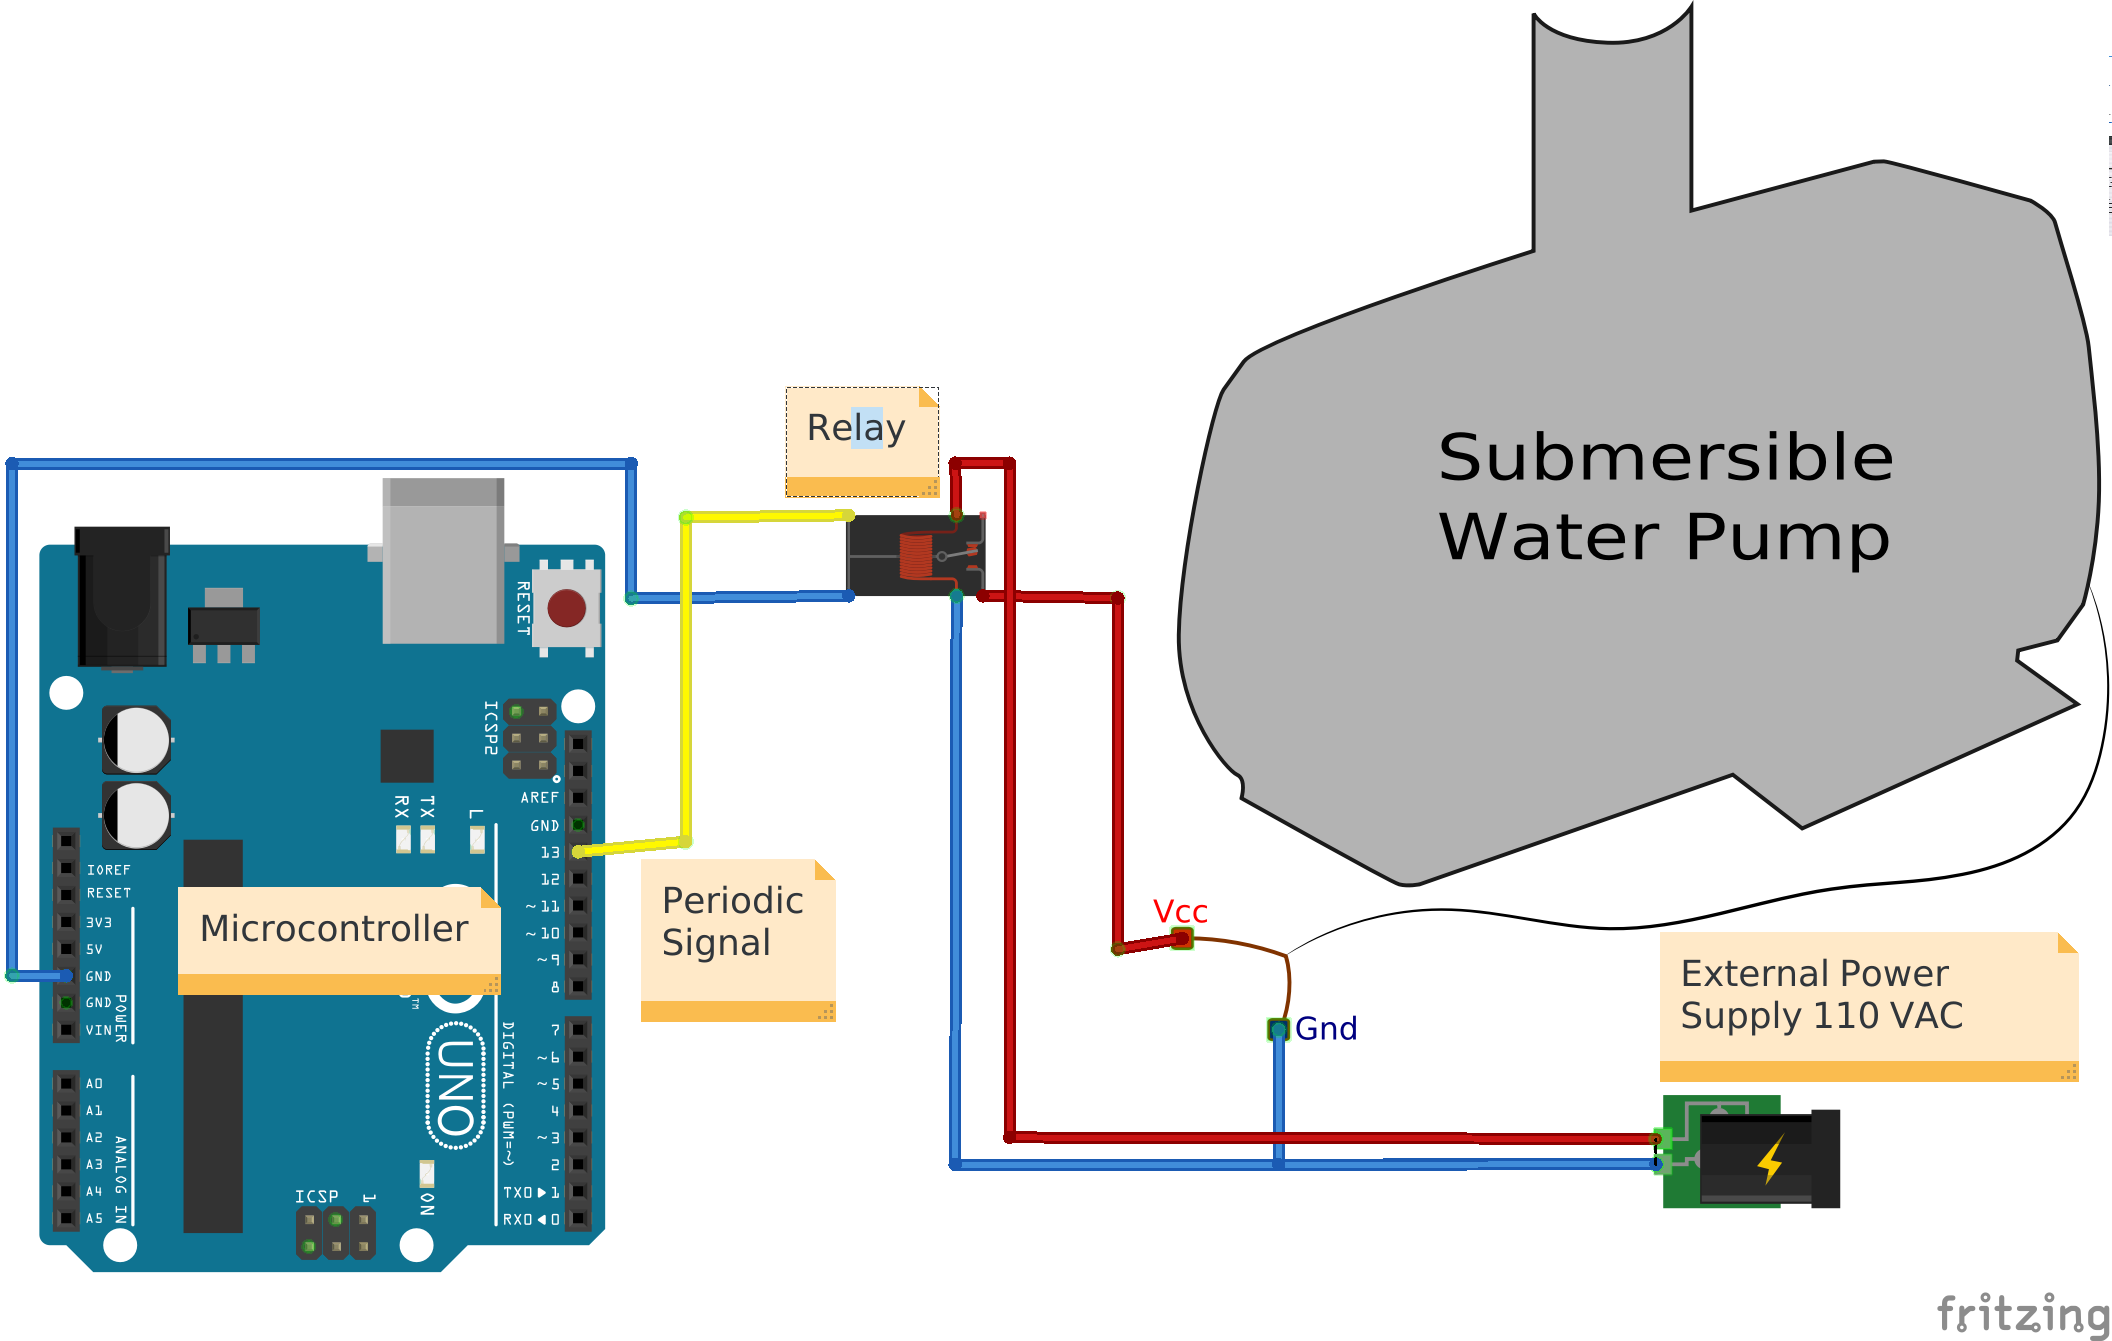
\includegraphics[width=.6\linewidth]{diagrams/architecture_bb}
    \caption{This diagram shows how the microcontroller interacts with the water pump}
    \label{fig:waterCycleDiagram}
\end{figure}

Each wire color has a meaning.
Blue represents the ground voltage,
red is high voltage
and yellow is low voltage.
The submersible water pump is located inside the fish tank and normally is turned off.
When the periodic signal comes from the microcontroller's digital output,
it is amplified by the relay switching,
which in turn makes the power supply to deliver high voltage to the water pump,
the latter works until the relay is switched again by the microcontroller's signal downtime.

\subsection{Project Decisions}
There are a lot of authors \cite{GoddekDelaideMankasinghEtAl2015} \cite{clark2009system} \cite{Leatherbury2014} that have had experience with Aquaponics automation.
Most of them chooses Arduino or Raspberry Pi as the main microcontroller.

Two great reasons for the Arduino's usage are:
This work's author already has an Arduino UNO,
but not a Raspberry PI.
Besides the main reference of this work,
the \cite{Kretzinger2015},
whose author has many years of experience with Aquaponics and its automation and he uses the Arduino as microcontroller.

The chosen components have been based in the references.
